
%(BEGIN_QUESTION)
% Copyright 2011, Tony R. Kuphaldt, released under the Creative Commons Attribution License (v 1.0)
% This means you may do almost anything with this work of mine, so long as you give me proper credit

Four solenoid-actuated block valves are used as safety shutoff devices for a petroleum pipeline, all of them signaled simultaneously by one ``logic solver'' controller.  The reliability rating ($R$) for each block valve -- describing its probability of faithfully obeying the signal from the logic solver -- is shown on the diagram:

$$\includegraphics[width=15.5cm]{i00218x01.eps}$$

Determine the {\it MooN} ratings for this four-valve block system, from the perspective of {\it dependability} (i.e. the {\it MooN} rating describing its ability to guarantee a shut-off pipeline), as well as from the perspective of {\it security} (i.e. the {\it MooN} rating describing its ability to guarantee a flowing pipeline).

\vskip 10pt

MooN (dependability) = \underbar{\hskip 50pt}  \hskip 70pt MooN (security) = \underbar{\hskip 50pt}

\vskip 50pt

Next, calculate the overall reliability that this four-valve block system will be able to guarantee shut-off of the pipeline, based on the individual reliability ratings given:

\vskip 10pt

$R_{shutoff}$ = \underbar{\hskip 50pt}

\underbar{file i00218}
%(END_QUESTION)





%(BEGIN_ANSWER)

{\it 2 points for each MooN answer, plus 6 points for the reliability calculation}

\vskip 10pt

MooN (dependability) = \underbar{\bf 3oo4}  \hskip 70pt MooN (security) = \underbar{\bf 3oo4}

\vskip 10pt

$R_{shutoff}$ = \underbar{\bf 0.98709}

%(END_ANSWER)





%(BEGIN_NOTES)

{\bf This question is intended for exams only and not worksheets!}

%(END_NOTES)


